

\section{Neutral dynamics in improved confinement MST plasmas}\label{sec:neutral_results}

The neutral dynamics are perhaps the most important factor in ion thermal transport in MST. As explained in previous sections in detail, the neutral dynamics can be difficult to measure directly, and physics-based modeling is needed. The inadequacy of inversion techniques and the need for physics simulation regarding neutrals has already been identified \cite{Eilerman2012}. There have been previous attempts to model the neutrals in MST using a Monte-Carlo simulation code called NENE, based on the principals set out by Hughes \textit{et al.} \cite{Hughes1978}. %Citation for NENE is here: https://doi-org.ezproxy.library.wisc.edu/10.1016/0021-9991(78)90045-1
NENE is similar to the DEGAS2 code that is used for this modeling work.
%How is NENE different from DEGAS2? What did it get wrong? Was it missing important physical processes in the neutral modelling? If so, which ones? Is there a justification for adding a 50eV neutral source in NENE given what you discussed earlier in terms of hot neutrals generated from charge exchange with plasma ions? -- MDN
%Clearified a bit more. --Xing
However, comparatively NENE did poorly for PPCD plasmas, and needed an \textit{ad hoc} 50eV uniform neutral source to improve the quality of fit\cite{Eilerman}. DEGAS2 improves upon NENE by offering a more complete set of physics interactions being simulated, especially around molecular dynamics such as molecular ionization, disassociation, and charge exchange, and well as better accounting of multi-step interactions that adds an effective $n_e$ dependence to impact ionization rate coefficients\cite{Stotler,Janev1984}. Further, the implementation of NENE on MST did not produce neutral temperature information, or the thermal effects of impact ionization, the importance of which becomes clear later in the section. The general setup of the neutral simulation within the model has been laid out previously in section \ref{sec:DEGAS2}, but before the density and temperature results can be discussed, we need to have a short detour to talk about fitting quality and the source geometry used to obtain the fits.

\begin{figure}
	\centering
	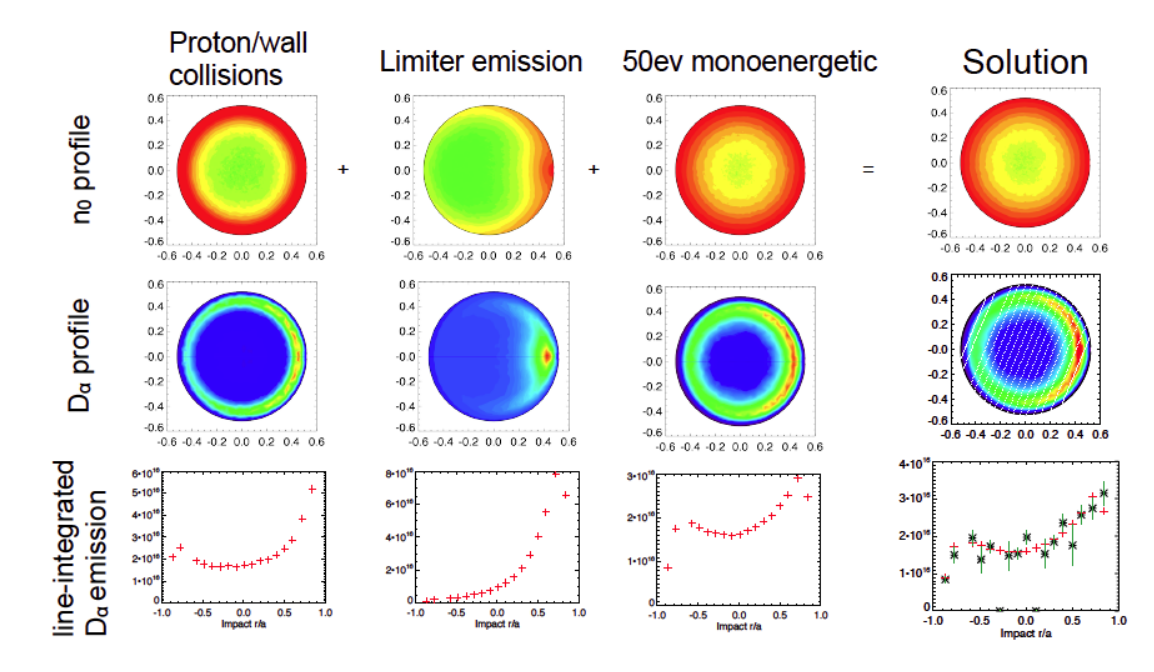
\includegraphics[width = 1.\linewidth]{ion_transport_results/nene_example.png}
	\caption[Example of NENE neutral output]{Example of NENE neutral output, the difference between this and the DEGAS2 results are examined in this section. (Reproduced from S. Eilerman's Thesis \cite{Eilerman})}\label{fig:nene_example}
\end{figure}

\subsection{Neutral source geometry, and fitting of observations}\label{sec:neutral_source_geometry}

In an ideal situation the neutral source rates would be known through direct observation and be modelled using the complete 3D geometry of the vacuum vessel. But as a practical matter, neutral recycling is complex and not within the scope of this work. Instead, a 2D neutral simulation is run with several independent neutral source profiles assuming toroidal symmetry. Each particle source has a defined geometry and rate. An instance of neutral analysis is simulated implementing each particle source independently, and then the rates are linearly fit to the observed $\dal$ emission levels (discussed in detail in section \ref{sec:DEGAS2}). Increasing the number of independent 'sources' via subdividing the wall geometry would give more fitting parameters, but the fitting problem becomes under constrained by the emission measurements, and the computational time needed increases unnecessarily. This work uses a three-source geometry as follows (illustrated in figure \ref{fig:DEGAS2_sources_and_density}):
\begin{figure}
	\centering
	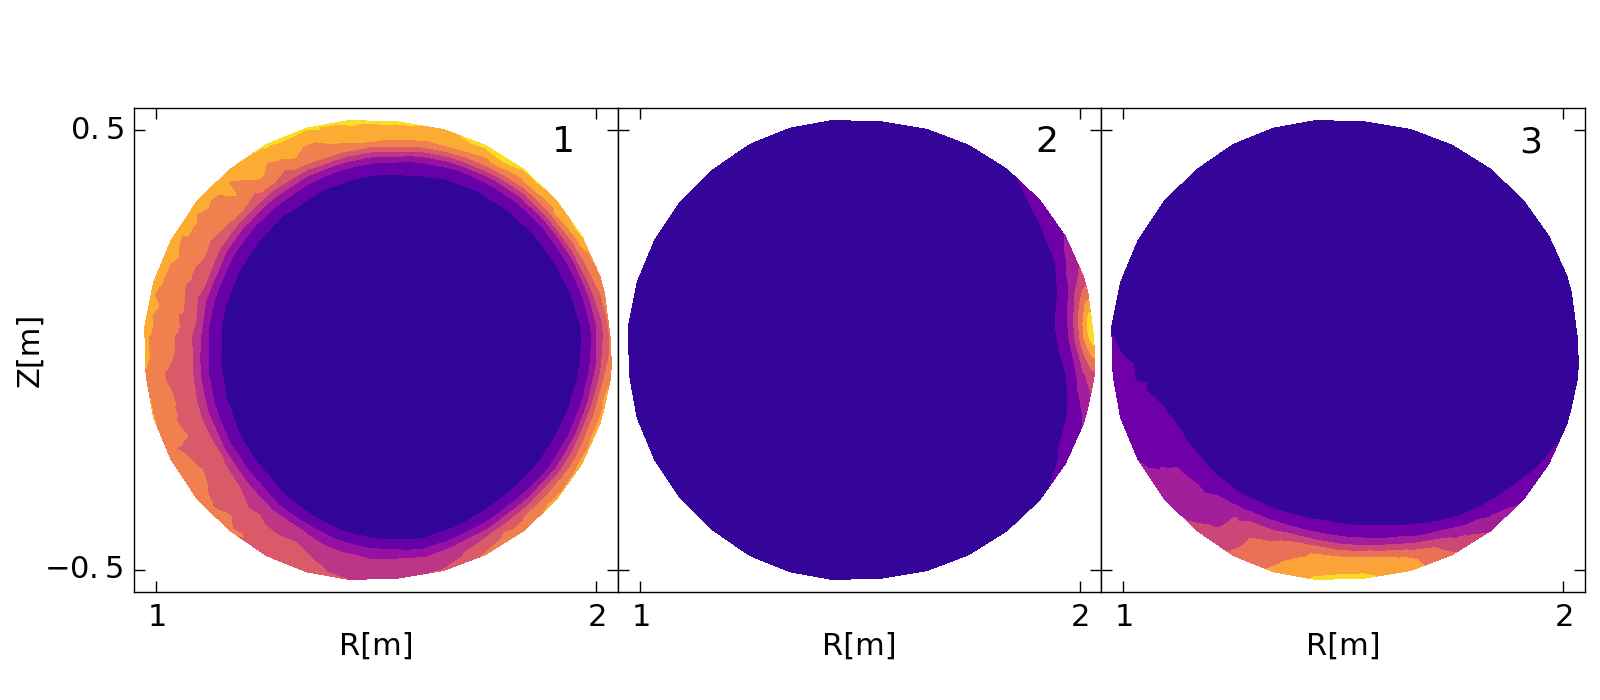
\includegraphics[width = 1.\linewidth]{ion_transport_results/source_comp.png}
	\caption[DEGAS2 source contributions]{Geometry of the normalized neutral density for the 3 sources used in DEGAS2. 1: 'Wall' source, 2:Limiter source, and 3: 'Duct' source. Details in text. It is interesting to point out that in the contribution from the 'uniform' source, there can be clearly observed the effect of the Shafronov shift on the neutral density. \textit{ie.} the neutral density 'hole' is correspondingly shifted to reflect the shift in the ionization region. This phenomenon is not seen in NENE results of the same source (figure \ref{fig:nene_example}), and it is unclear why. Though likely related to self-consistency issues in implementation.}\label{fig:DEGAS2_sources_contrib}
\end{figure}
\begin{enumerate}
    \item A poloidally uniform source representing the walls of MST, with the exception of the area detailed in the following source. 
    \item A poloidally localized source corresponding to the location of the outboard limiter. The outboard limiter (typically) defines the LCFS on MST and is known to be a major source of recycling as well as impurities.  
    \item A poloidally localized source corresponding to the bottom 45\textdegree of the wall. This is the location of the pumping duct and gas injection valves of MST. 
\end{enumerate}
The contributions from each source (to density, for example) are treated as linearly independent. This is due to the fact that neutral-neutral collisions are very rare compared with neutral-ion and neutral-electron collisions at typical parameters. Typical contributions from each source are shown in figure \ref{fig:DEGAS2_sources_contrib}. This project began by considering only the first two sources, with the second extending uniformly around the circumference of the vessel poloidal cross section. However, it is found that in some instances the first two source terms could not be used to explain measurements from the $D_\alpha$ array. In particular, the intensity on the central view chords would be systematically under-predicted by the code. By hypothesizing that the neutral population may have a vertical asymmetry due to preferential sources and sinks in the lower region of the vessel. This is the location of the pumping duct and all of the fueling gas injection valves. If this region has a different effective source rate than 'the rest of the wall', the code is then able to give a better fit to the observations. (see figure \ref{fig:DEGAS2_source_comp})%, and \ref{fig:DEGAS2_typical_fit}). Additionally, it is useful to point out that

\begin{figure}
	\centering
	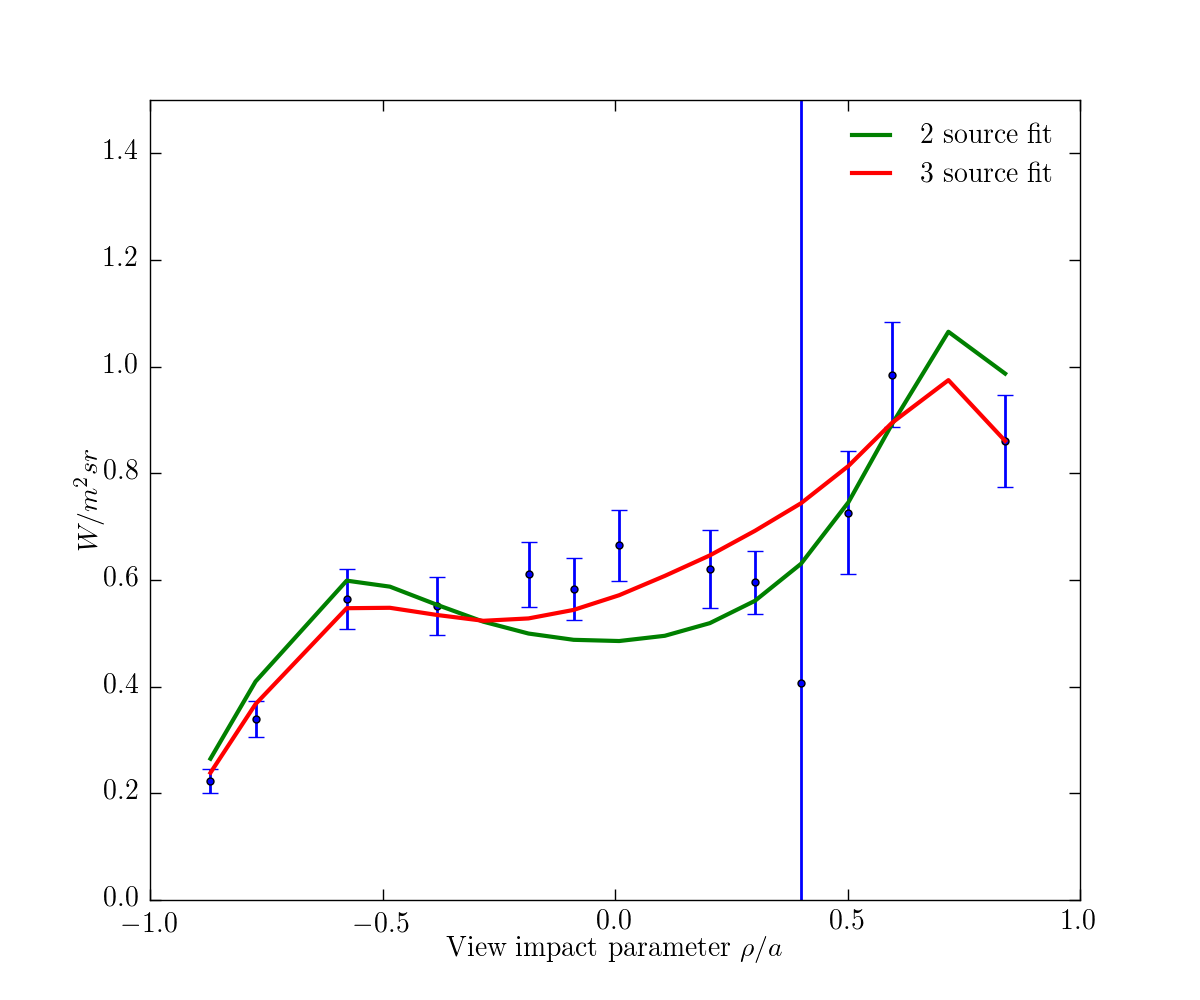
\includegraphics{ion_transport_results/source_comparison.png}
	\caption[Comparison between 2 source and 3 source fit for DEGAS2]{Comparison between 2 source and 3 source fit for DEGAS2.}\label{fig:DEGAS2_source_comp}
\end{figure}

\begin{figure}
    \centering
    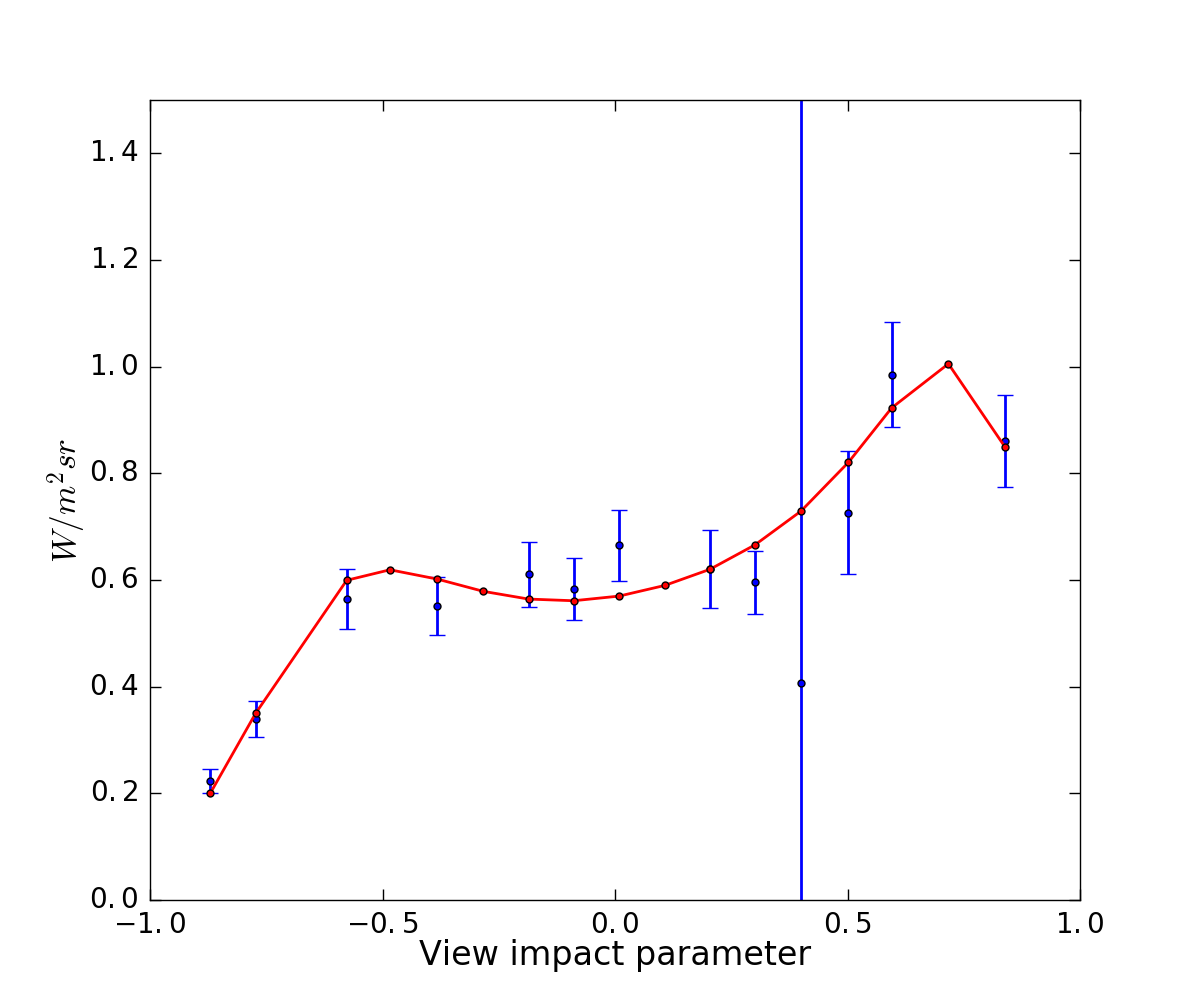
\includegraphics{ion_transport_results/DEGAS2_typical_fit.png}
    \caption{A typical DEGAS2 fit of ensembled $\dal$ signal.}
    \label{fig:DEGAS2_typical_fit}
\end{figure}

\subsection{Neutral density in PPCD}

\begin{figure}
    \centering
    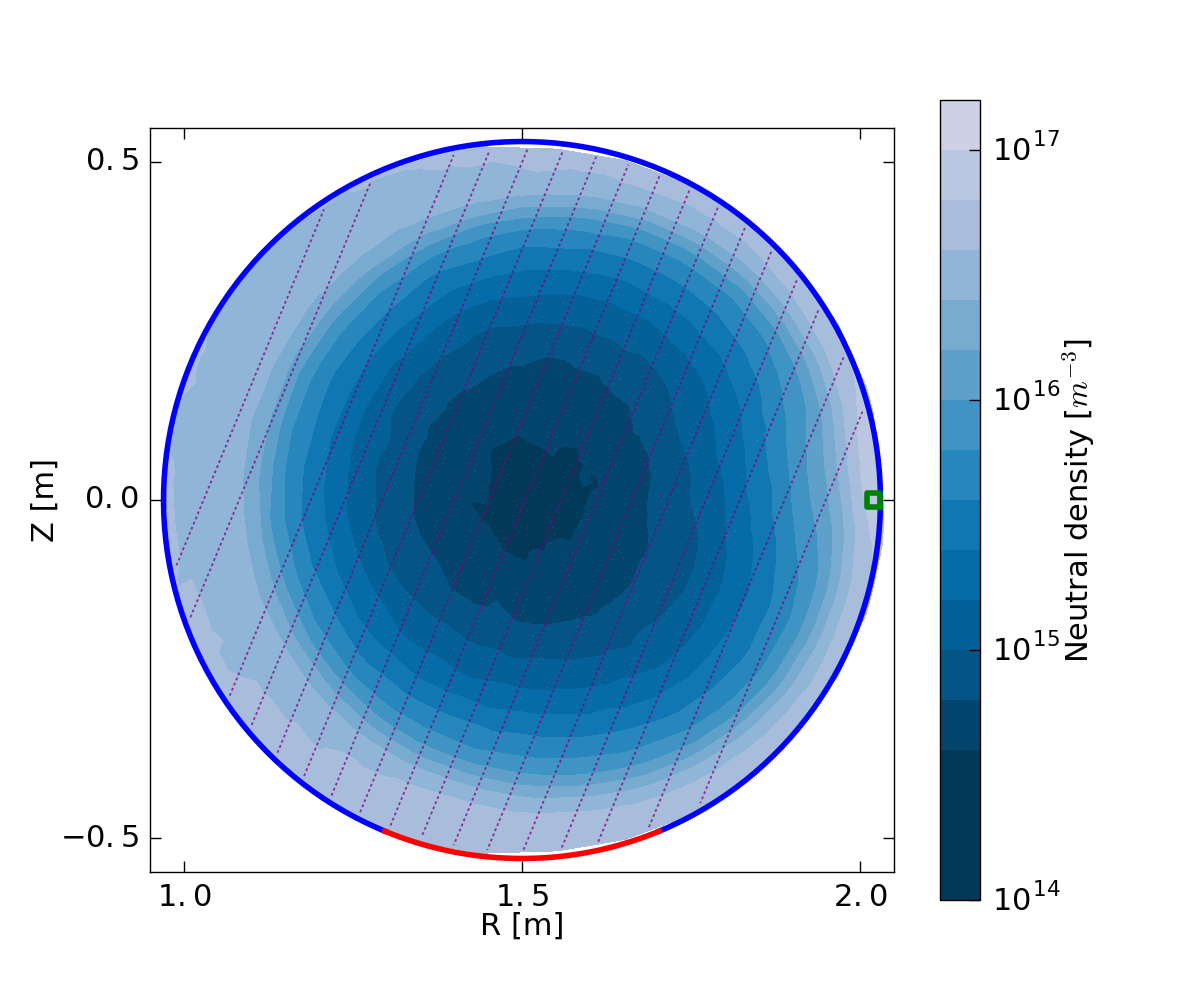
\includegraphics{ion_transport_results/DEGAS2_density2d.png}
    \caption[Neutral density via DEGAS2]{Neutral density via DEGAS2 simulation, with the geometry of the three sources overlayed. Using the numbering presented in section \ref{sec:neutral_source_geometry}: source 1 is in blue, source 2 is in green, and source 3 is in red. The dashed lines represent the location of the available views.}
    \label{fig:DEGAS2_sources_and_density}
\end{figure}

\begin{figure}
    \centering
    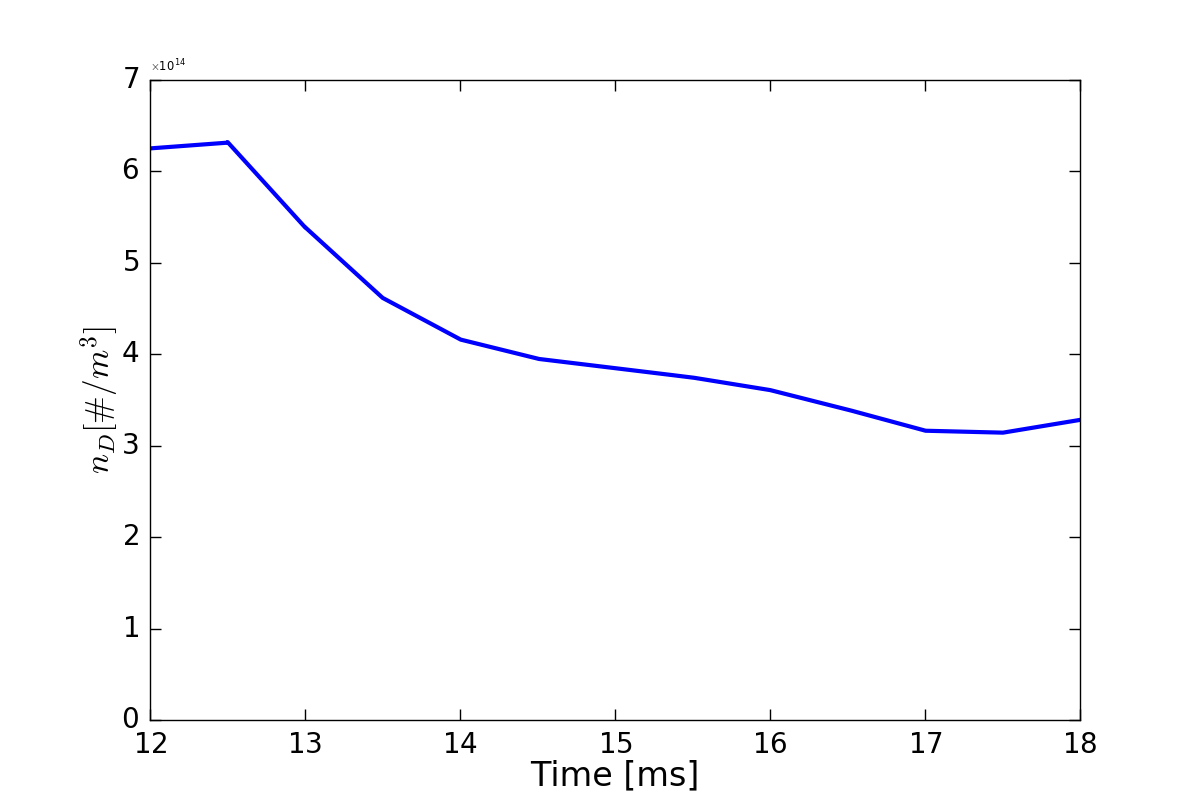
\includegraphics[width=0.8\linewidth]{ion_transport_results/neutral_vs_time.png}
    \caption[Core neutral density over time]{Core neutral density over the time span of the PPCD period. This result is from the ensemble of good PPCD shots analyzed.}
    \label{fig:neutral_vs_time}
\end{figure}

Unsurprisingly, the neutral density is edge dominated and decreases by about 2.5 orders of magnitudes as one 'travels' towards the core. The details can be seen in figure \ref{fig:DEGAS2_sources_and_density} and \ref{fig:DEGAS2_power_1d}. The edge neutral density is comparable with previous estimates, but the core density is about 1/4 of previous calculations using the NENE code~\cite{Ei}. % This comparison of the NENE and DEGAS2 code predictions for neutral density profiles that best fit observed neutral emission measurements doesn't really explain which model is more believable. Aside from the ad-hoc 50eV source, what are the differences between the two codes? 
%Added more on the improvement DEGAS2 makes in first paragraph of section. -Xing
Though when NENE is run for my particular shot ensemble, it returns results lower than that presented, and the core density from DEGAS2 is ~ 55\% of NENE. As pointed out above, the DEGAS2 fit have the advantage of not relying on an \textit{ad hoc} 50eV neutral source to achieve the fit, and the neutral density more self consistently show the effect of the Shafronov shift (see also figure \ref{fig:DEGAS2_sources_contrib}). 
Further, the neutral density in PPCD is not entirely constant; the early part of PPCD sees the neutral density decreasing until around 16.5ms when it stabilizes until the end of PPCD (figure \ref{fig:neutral_vs_time}. This neutral density estimates is also in line with that from s. Kumar's measurement of Al charge state fractions in the core. The charge state fraction of Al$^{11+}$ to Al$^{13+}$ is very sensitive to neutral density as the charge exchange process keep the Al$^{13+}$ population down. DEGAS2's estimate of core neutral density. The DEGAS2 neutral density is still too might to match that needed by J. Waksman to explain the NBI heating effects observed. However, this is perhaps not a good direct comparison as his work are on well optimized low current (200kA) PPCD, which, other than the problem of differing plasma current as my parameters, is inherently difficult for $\dal$ observations to constrain neutral density as the emission measurements begin to approach noise levels of the detector. 

\begin{figure}
    \centering
    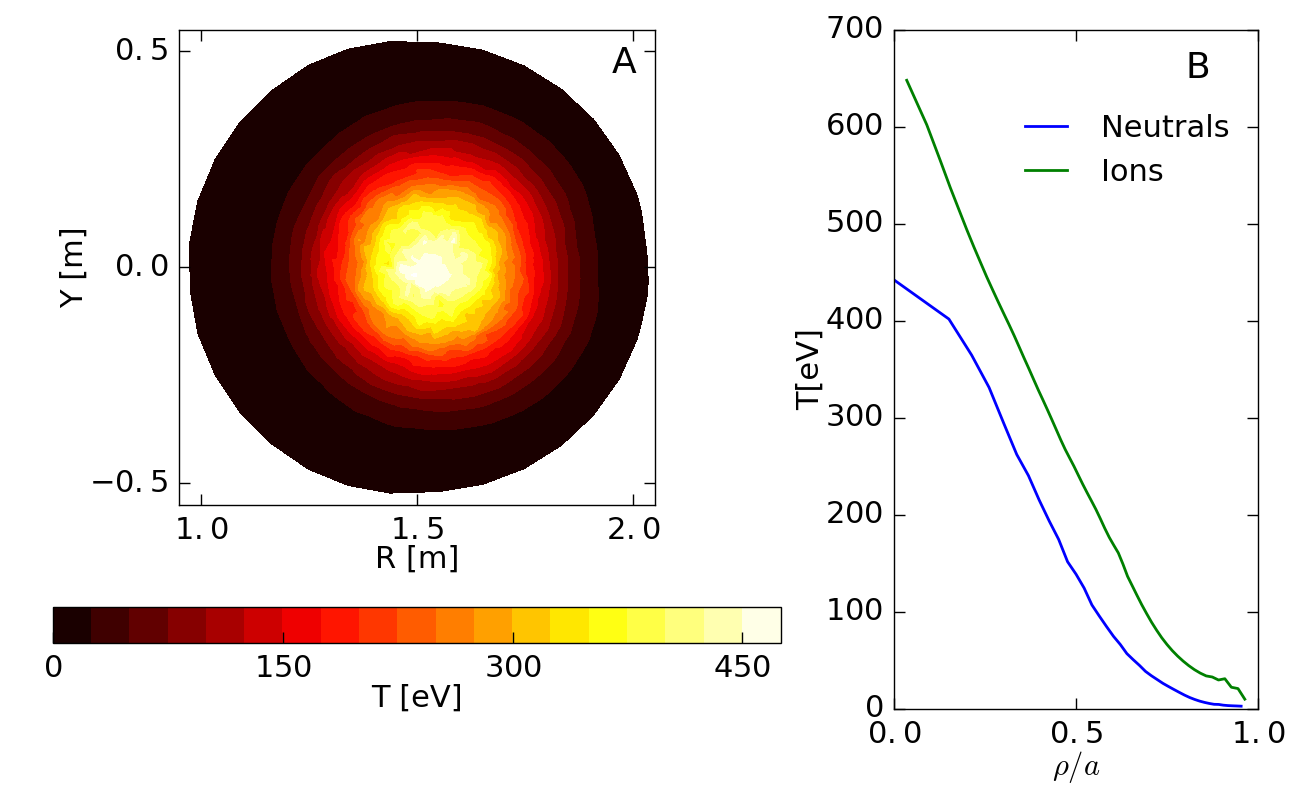
\includegraphics[width=\linewidth]{ion_transport_results/DEGAS2_temperature2d.png}
    \caption[Neutral temperature via DEGAS2]{Neutral temperature via DEGAS2 simulation. A) The 2-d temperature results. B) The flux surface averaged results, with $T_i$ for comparison.}
    \label{fig:DEGAS2_temperature}
\end{figure}

Another notable improvement of the understanding of the neutral dynamics is the neutral temperature information provided by DEGAS2. Though it may not be immediately obvious, but a high $T_{\text{neutral}}$ is needed for the neutrals to penetrate into the plasma volume. The mean free path of a 'room temperature' neutral is very short in MST parameters, and neutrals created by charge exchange reactions, and a small amount of Frank-Condon neutrals from energetic disassociation of D$_2$ would dominate the neutrals interior to the plasma. This is reflected by the DEGAS2 results (figure \ref{fig:DEGAS2_temperature}). Notably, the neutral temperature is a significant fraction of the ion temperature, meaning that only a fraction of the ion's thermal energy is effectively lost in a charge exchange reaction.

\subsection{Charge exchange, impact ionization, and ion source rate}

\begin{figure}
    \centering
    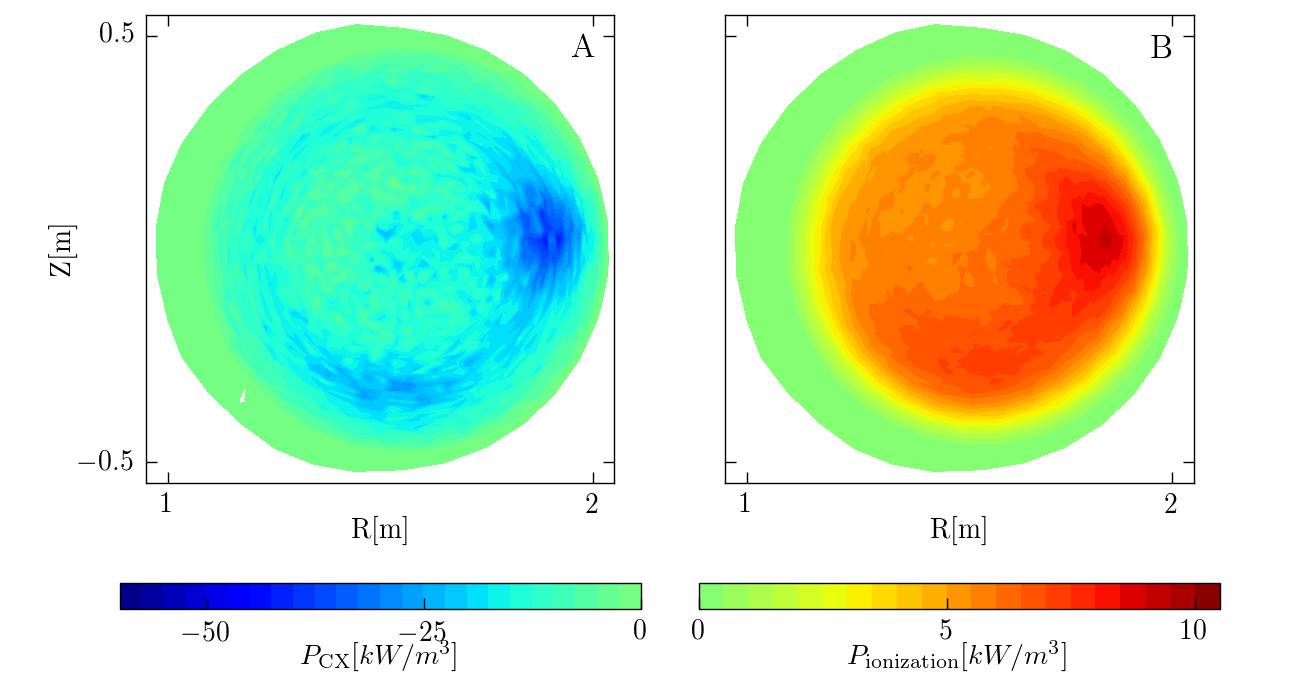
\includegraphics[width=\linewidth]{ion_transport_results/DEGAS2_power_terms_2d.png}
    \caption[DEGAS2 charge exchange and impact ionization terms]{DEGAS2 2D  A) charge exchange and B) impact ionization terms. Note the difference in the color bar range. Less obviously, the up/down asymmetry is also present in this plot. This result is from ensembled PPCD shots at 15ms.}
    \label{fig:DEGAS2_power_2d}
\end{figure}

\begin{figure}
    \centering
    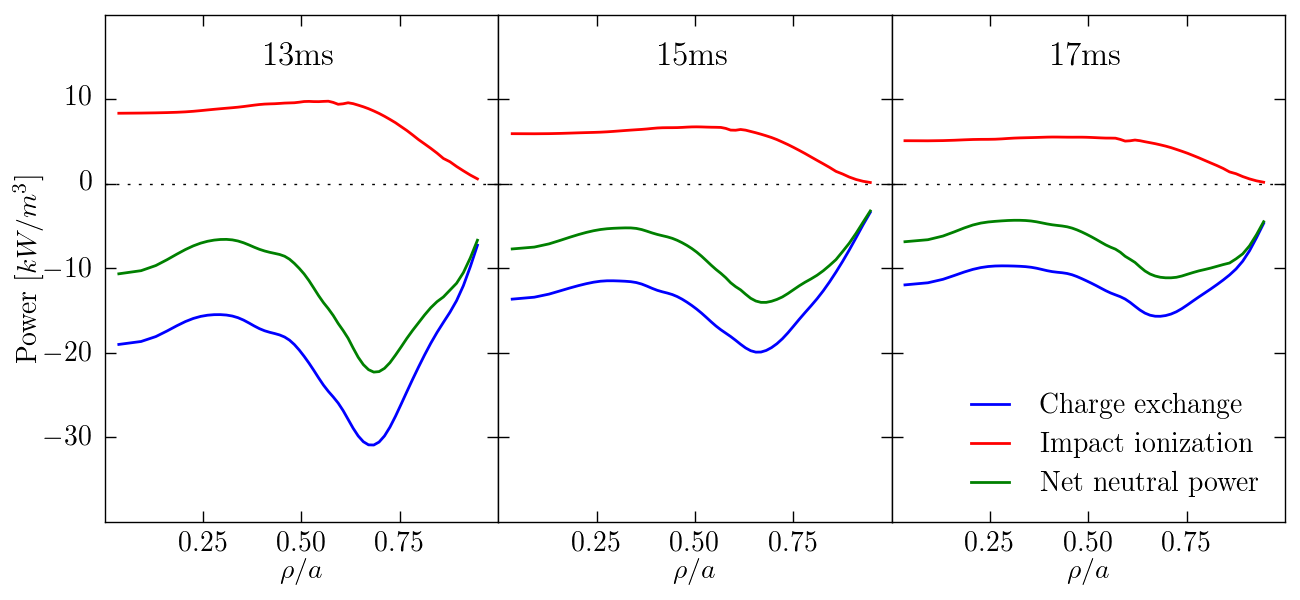
\includegraphics{ion_transport_results/DEGAS2_power_terms_1d.png}
    \caption[1-D neutral power terms]{1-D neutral power terms at 13ms, 15ms, and 17ms. The 'net neutral power' refers to the sum of the two terms, as electron impact ionization is a process that recovers some thermal energy from the neutrals fluid.}
    %This plot should include 'net charge exchange loss'
    \label{fig:DEGAS2_power_1d}
\end{figure}


The charge exchange loss rate displays an hollow profile that is significantly skewed outboard, like the ion density. However, the poloidal transit time are small on the RFP and neutral effect on the majority ion fluid is still considered on a flux surface averaged basis despite significant asymmetry. On a practical basis, this hollow profile is the creation of the declining neutral density towards the core, and the increasing majority density as well as temperature difference. The trend of declining neutral density also translates to the charge exchange loss as expected. The electron impact heating is an interesting to consider as it represents a partial 'recovery' of the thermal energy lost in charge exchange (details in section \ref{sec:neutral_physics}). However, as the neutral's temperature is below that of majority ion, this actually results in temperature decrease. In general, I use 'heating' to describe thermal energy input into the ion fluid which does not necessarily increase the temperature. 

\begin{figure}
    \centering
    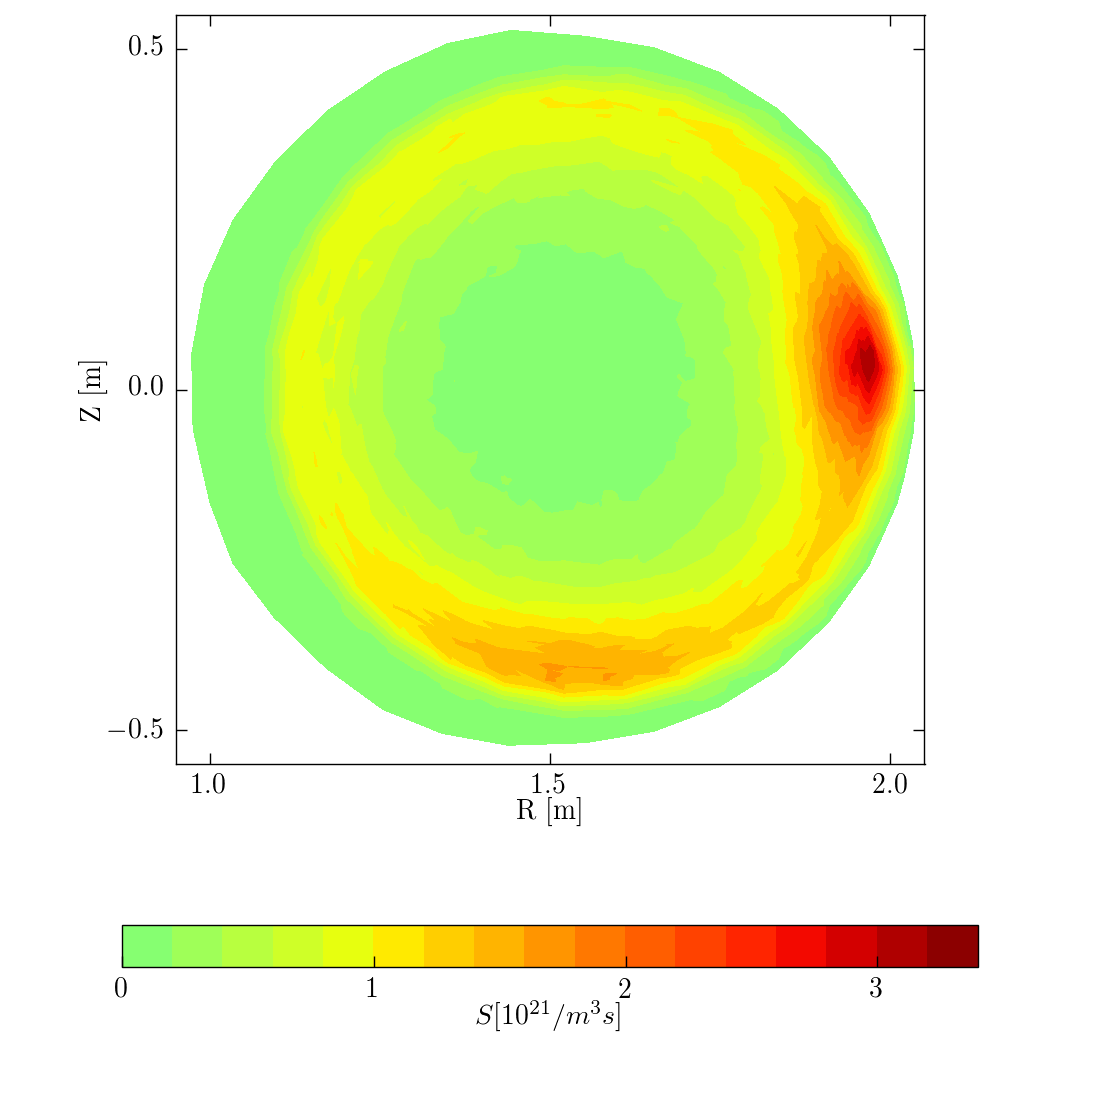
\includegraphics{ion_transport_results/source_2d.png}
    \caption{DEGAS2 ion source rate results.}
    \label{fig:DEGAS2_source_rate}
\end{figure}

The ion source rate also displays the same characteristics as the power terms. However, it is significantly more hollowed out since it does not depend on the difference in ion and neutral temperature, which is higher in the core. This means that the ion source rate is not sufficient to explain the density rise in the core. The consequence of this is to hint at an inward pinch mechanism to be explained in more detail in section \ref{sec:eb_pinch}

%\subsection{Unintuitive model response of \textit{ad hoc} heating in the edge}
%\begin{figure}
%    \centering
%    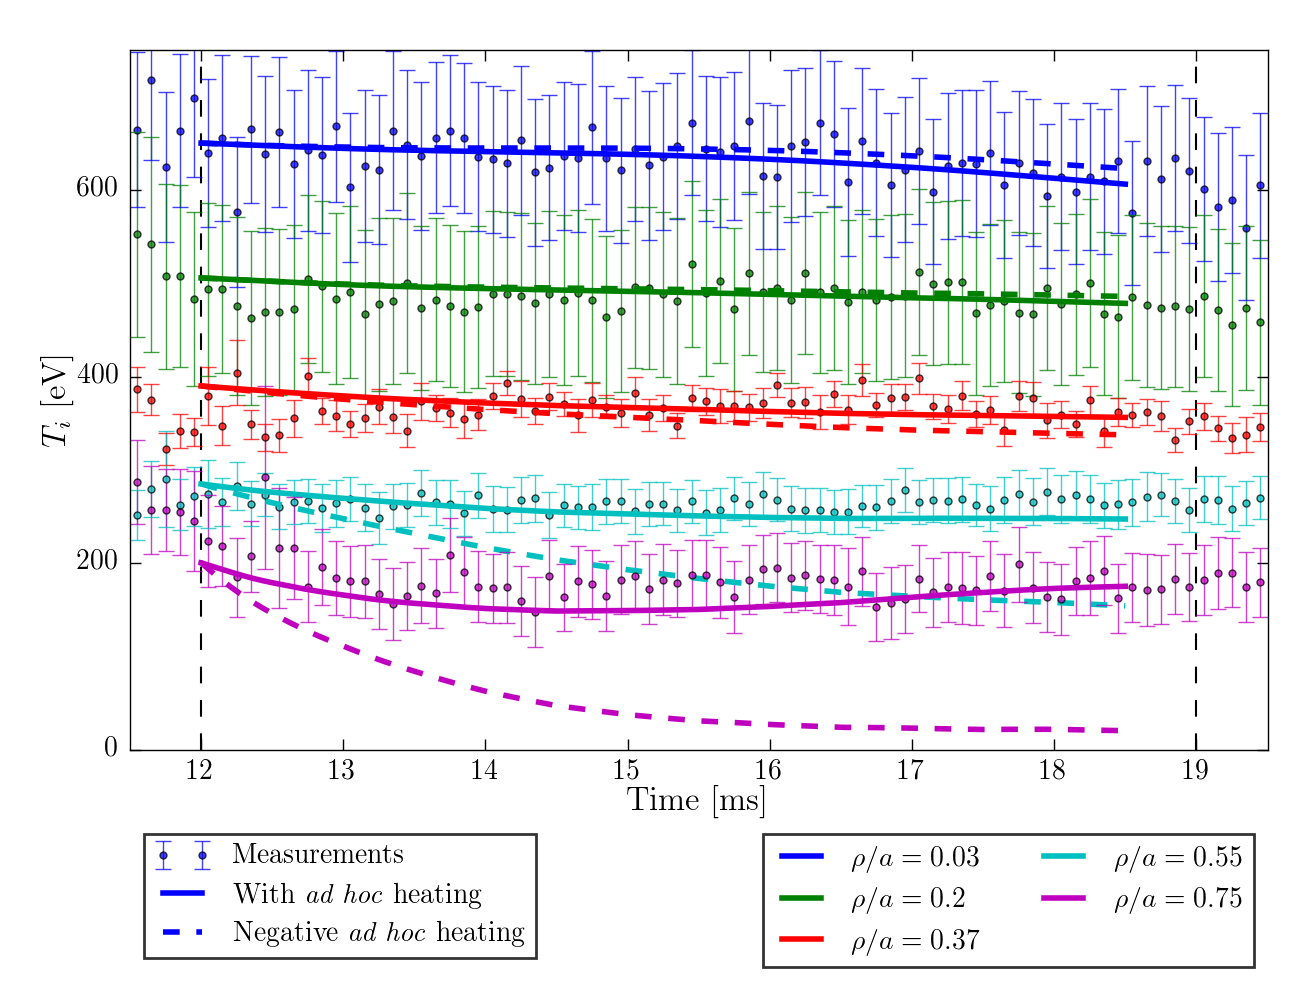
\includegraphics[width=\linewidth]{ion_transport_results/unintuitive_response.png}
%    \caption{The effect of having a low ion temperature edge on charge exchange}
%    \label{fig:unintuitive_cx_response}
%\end{figure}

%During the adjustment process for the model, it became clear that ion heating in the edge have an effect on the charge exchange loss in the core through it's effect on ion temperature. Suppose you have an edge region where the ion temperature is only a few eVs, but the electrons are on the order of 50 to 100 eV. In this region, electron impact ionization of neutrals would dominate charge exchange, and any neutral particle entering the plasma would more likely be ionized before undergoing charge exchange, thus decreasing the neutral penetration. The decreased penetration would in turns result in a more hollowed out neutral density, as well as charge exchange loss and ion source rate. This situation was created in the model from a mistake in the calculation in the flow effects in the edge, and when \textit{ad hoc} heating is applied this erroneous model to bring it inline with the observed temperature without changing how the rest of the model is calculated, the core temperature is predicted to be lower. However, this effect seems most significant when the edge ion temperature drops to ~10eV or lower for a significant radius. When the mistake was corrected, the model predicted edge ion temperature of ~50eV at $\rho_v/a \approx 0.75$ without \textit{ad hoc} heating terms, and increasing it to the observed ~175eV using \textit{ad hoc} heating only dropped the core temperature very slightly.

